\subsection*{Assignment 2.e \hrule}
\textbf{Question}
\begin{quote}
Repeat the previous exercise for 1000 haloes each containing 100 satellites. Make another log-log plot showing $N(x) = n(x)4 \pi x^2$ over the same range as before, but now over-plot a histogram showing the average number of satellites in each bin. Use 20 logarithmically-spaced bins between $x = 10^{-4}$ and $x_{max}$ and don't forget to divide each bin by its width. Do you generated galaxies match this distribution?
\end{quote}


\textbf{Solution}
\begin{quote}
The histogram with the average number of satellites is created by first creating a histogram for each halo and adding each of these histograms together. The obtained "super" histogram is next divided by the width of the bins to correct for the different sized bins. The bin width corrected "super" histogram is finally divided by the number of halos to obtain the histogram with the average number of satellites. 

The code that generates the radii and the histogram is located in the file: \textsf{./code/assignment2\_ e.py}. The content of this file and its output can be found below\footnote{The code of the helper functions used in this file can be found in the previous assignment.}. The output is located at

\end{quote}
  
\textbf{Code - plots}
\begin{quote}
\lstinputlisting{./code/assignment2_e.py}
\end{quote}

\textbf{Output - plot}

\begin{quote}
The output generated by \textsf{./code/assignment2\_ e.py} consists of figure \ref{fig:sat} on the next page.
\newpage
\begin{figure}[!ht]
\centering
\vspace*{-1cm}
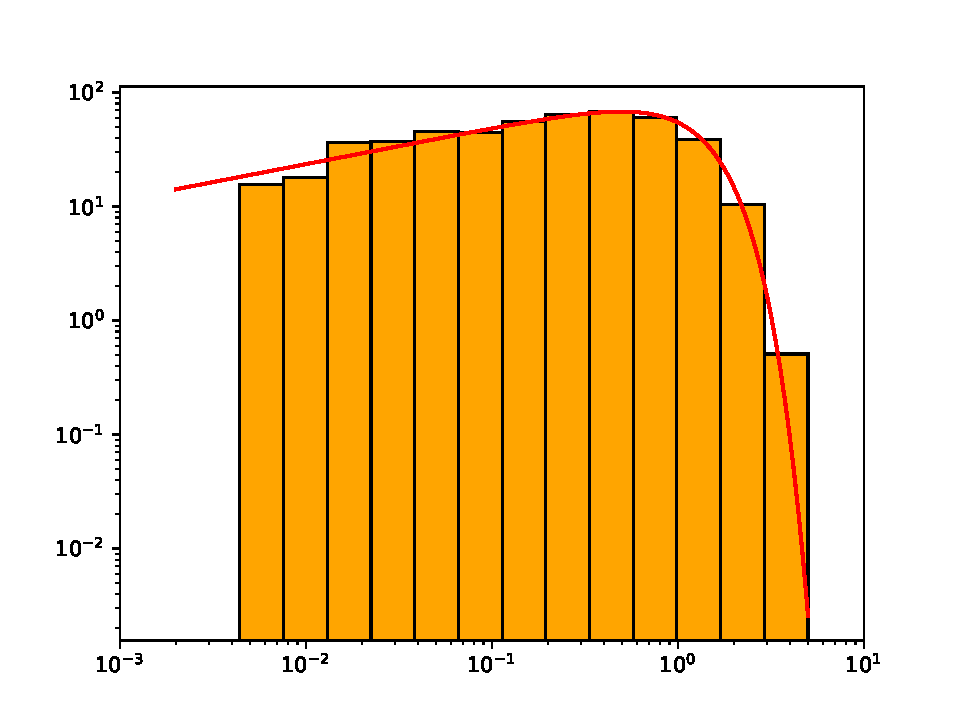
\includegraphics[width=12cm, height=8.5cm]{plots/assignment2e.pdf}
\caption{The average number of satellites on a spherical shell at distance $x = r/r_{viral}$. The red line is the original function $N(x)$ that is used to generate the histogram.}
\label{fig:sat}
\end{figure}
\end{quote}











